\begin{figure}[ht]
  \begin{centering}
    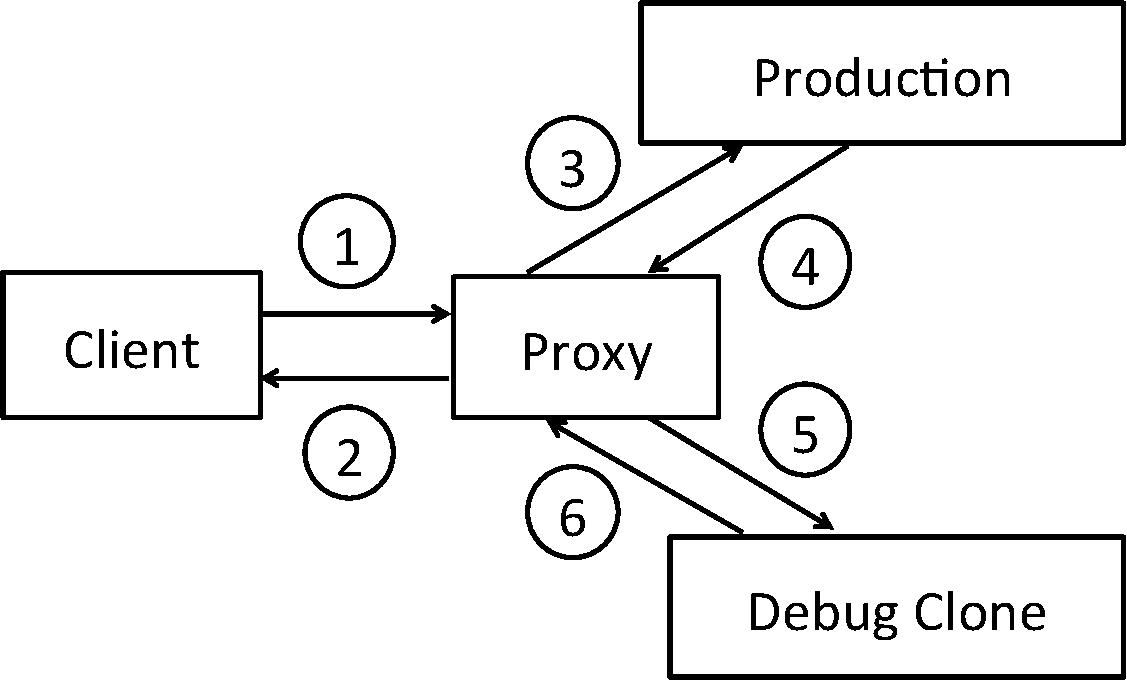
\includegraphics[width=0.4\textwidth]{figs/network_dup.pdf}
%    \captionsetup{justification=centering}
    \caption{Network Duplicator: Thread 1 sends traffic on links 1 and 3, Thread 2 manages links 2 and 4, Thread 3 forwards traffic on link 5, \& Thread 4 reads and drops data on link 6}
    \label{fig:duplicator}
  \end{centering}
\end{figure}

%\vspace{-0.25cm}
\subsection{Proxy Network Duplicator} 
\label{sec:proxyDuplicator}


\xxx{Why do we describe the synchronous approach at all? I think it's obvious that it's not the right one. Would rather hear more about *what* we did, rather than *why* (There will be reviewers who say 'duh' to the why)}

In order for \textit{live debugging} to work, both production and debug containers must receive the same input.
A major challenge in this process is that the production and debug container may execute at different speeds (debug will be slower than production): this will result in them being out of sync.
Additionally, we need to accept responses from both servers and drop all the traffic coming from the debug-container, while still maintaining an active connection with the client.
Hence simple port-mirroring and proxy mechanisms will not work for us.

Our solution is a customized TCP level proxy. 
This proxy duplicates network traffic to the debug container while maintaining the TCP session and state with the production container. 
Since it works at the TCP/IP layer, the applications are completely oblivious to it.

To understand this better let us look at Figure~\ref{fig:duplicator}: Here each incoming connection is forwarded to both the production container and the debug container . 
Where data is sent from the client to the proxy (link 1), then from proxy to production (link 3), and finally from proxy to debug container (link 5). 
Replies are received from production to proxy(link 4), and forwarded to the client (link 2), whereas replies from debug container to proxy (link 6), are simply dropped. 

TCP is a connection-oriented protocol and is designed for stateful delivery and acknowledgment that each packet has been delivered.
Packet sending and receiving are blocking operations, and if either the sender or the receiver is faster than the other the send/receive operations are automatically blocked or throttled.

This can be viewed as follows: Let us assume that the client was sending packets at $X Mbps$ (link 1), and the production container was receiving/processing packets at $Y Mbps$ (link 3), where $Y<X$. 
Then automatically, the speed of link 1 and link 2 will be throttled to $Y Mbps$ per second, i.e the packet sending at the client will be throttled to accommodate the production server. 
Network throttling is a default TCP behavior to keep the sender and receiver synchronized.
However, if we also send packets to the debug-container sequentially in link 5 the performance of the production container will be dependent on the debug-container. 
If the speed of link 5 is $Z$ $Mbps$, where $Z < Y$, and $Z < X$, then the speed of link 1, and link 3 will also be throttled to $Z$ $Mbps$.
The speed of the debug container is likely to be slower than production: this may impact the performance of the production container.

To avoid a slowdown in the production container, we use 4 threads T1, T2, T3, T4  to manage each incoming connection to the proxy.
Thread T1 forwards packets from the client to the proxy (link 1), and from the proxy to the production container (link 3). 
It then uses a non-blocking send to forward packets to an internal pipe buffer shared between thread T1, and thread T3.
Thread T2 reads the responses from the production container and forwards them to the client (link 4 and 2).
Thread T3 then reads from this piped buffer and sends the  traffic forward to the debug-container( link 5), while Thread T4, receives packets from the debug-container and drops them (link 6).

The above strategy allows for non-blocking packet forwarding and enables a key feature of \parikshan, whereby it avoids slowdowns in the debug-container to impact the production container.
We take the advantage of an in-memory buffer, which can hold requests for the debug-container, while the production container continues processing as normal.
A side-effect of this strategy is that if the speed of the debug-container is too slow compared to the packet arrival rate in the buffer, it may eventually lead to an overflow. 
We call the time taken by a connection before which the buffer overflows it's \emph{debug-window}.
We discuss the implications of the \emph{debug window} in Section \ref{sec:window}.  
